tinylang的项目布局遵循了我们在第2章,LLVM源的访问中列出的方式。每个组件的源代码在lib目录的子目录中,而头文件在include/tinylang的子目录中,子目录以组件命名。在第2章,我们只创建了基本组件。\par

在前一章中,我们知道需要实现词法分析器、解析器、AST和语义分析器。其都有自己的组件,称为Lexer、Parser、AST和Sema。上一章中使用的目录布局如下:\par

\hspace*{\fill} \par %插入空行
\begin{center}
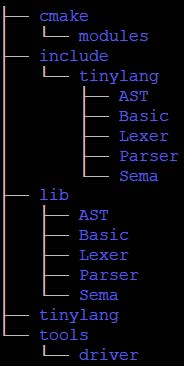
\includegraphics{content/2/chapter4/images/1.jpg}\\
图4.1 – tinylang项目的目录布局
\end{center}

组件有明确定义的依赖项。在这里,Lexer只依赖于Basic。Parser依赖于Basic、Lexer、AST和Sema。最后,Sema只依赖于Basic和AST,这些定义良好的依赖有助于对组件的重用。\par

让我们仔细了解一下它们是如何实现的。\par































































































